% cambiamenti nello pseudocodice
\chapter{Implementation}
Pseudo-code has been modified fixing some logic flaws, in particular:
\begin{itemize}
	\item Manage packet coming from servers to clients, in that case always install a forward rule, server is always trusted
	\item Checking for connection coming from clients to new server address must be done only when protection is enabled.
	\item The dictionary of clients connections must be cleared when connection to new server address is detected
\end{itemize}

\begin{figure}[H]
\begin{center}
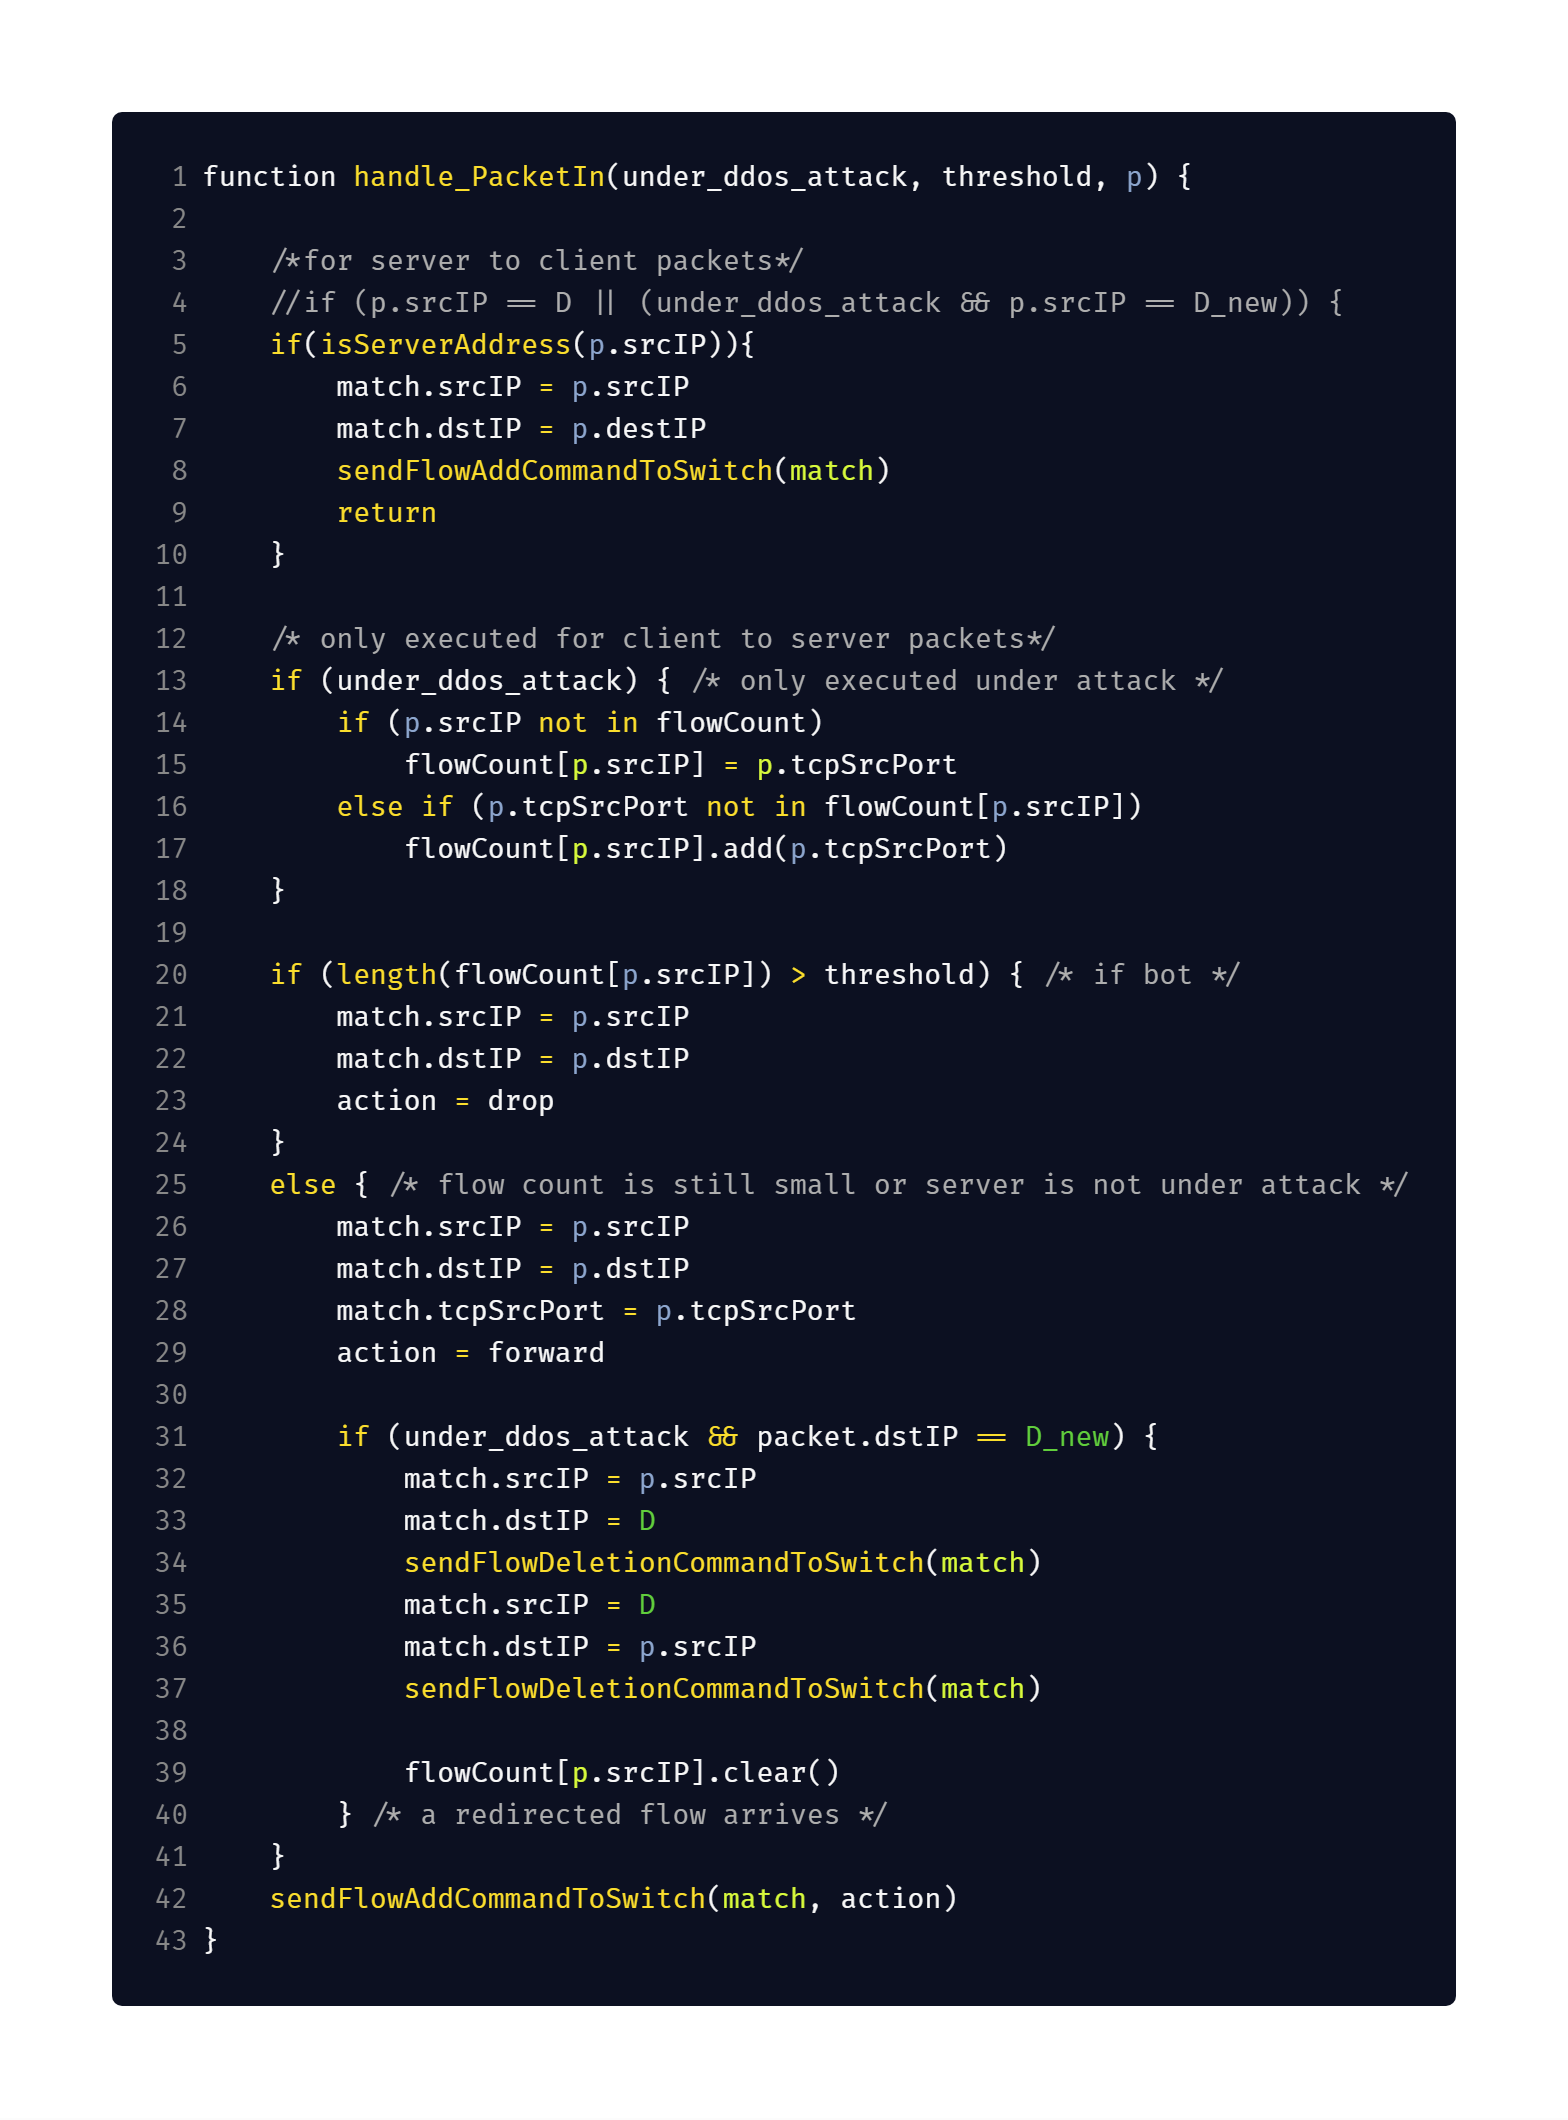
\includegraphics[width=0.8\textwidth]{images/pseudo_code_corrected.png}
\label{fig:pseudocode}
\caption{Controller corrected pseudo-code}
\end{center}
\end{figure}

\chapter{Learning Switch}
As stated on the Requirements chapter about Learning Switch, we needed only to modify the already existing \textit{ILearningSwitch} interface adding the already existing \textit{LearningSwitch} public method called \textit{getFromPortMap()}. However this was not sufficient to solve all the problem related to the coexistence of both LearningSwitch and DDoSDefence controller rules.

One of the first solution was to set all the DDoSDefence controller flow table rules to the highest priority (so higher than LearningSwitch ones), however, in some occasions, in particular when DDoSDefence controller rules was expiring, LearningSwitch ones were predominating.

To solve the problem, we decided to modify the implementation of LearningSwitch to set ``switching'' rules only for ARP and ICMP packets. This time we set an higher priority for LearningSwitch pipeling order to let the controller autolearn port-MAC entries before the execution of DDoSDefence controller, which will use this entries to set forward rules.

% parte iniziale del testing
\chapter{Testing}
\begin{figure}[H]
\begin{center}
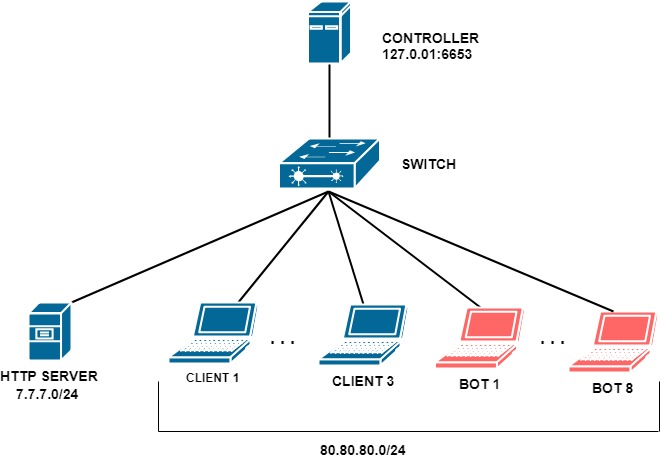
\includegraphics[width=0.8\textwidth]{images/TestingTopology_new.jpg}
\label{fig:pseudocode}
\caption{Controller corrected pseudo-code}
\end{center}
\end{figure}

We made some refining to the test topology names to best describe all the system parts. No change have been done on ip subnets or topology type.

At the beginning, we decided to use \textit{mininet CLI} for making that simple topology, however this turned out to be an issue because it was not possible to automatically inject console commands on each single client. At the end, we decided to write a custom python script using \textit{mininet} python library.

The script provides a GUI, can execute enable protection procedure on behalf of server (through console command injection). It uses \textit{requests} library for executing REST API requests (for initialization and enable protection). The GUI displays one console for each Client/Bot where each of them reports their HTTP request results. GUI can also display OpenFlow Switch flow table entries.
A set of buttons is provided to start the the test, enable the protection and doing some other generic tests (like ping).

% difficoltà incontrate
\chapter{Implementation Issues}
\paragraph{Execution order of floodlight modules}
As stated on the course slides, floodlight module order was defined by a particular file into the source folder. However this turned out to be different in the latest version of \textit{floodlight} where module order must be specified using two controller methods, which are \textit{isCallbackOrderingPrereq()} and \textit{isCallbackOrderingPostreq()}. \footnote{{https://floodlight.atlassian.net/wiki/spaces/floodlightcontroller/pages/1343513/How+to+Write+a+Module\#HowtoWriteaModule-OrderingModuleswhenProcessingOpenFlowMessages}}

\paragraph{NORMAL rule (action.normal)}
\textit{Normal} rule works only for hybrid switches, and \textit{OpenVirtualSwitch} is not one of them. This led to reimplement the L2 switch functionalities using \textit{LearningSwitch} implementation. \footnote{https://www.opennetworking.org/wp-content/uploads/2014/10/openflow-spec-v1.3.3.pdf}

\paragraph{Deleting flow rule types}
To delete one or more OpenFlow rules it is required to use one of these \textit{OFFlow} types: \footnote{https://floodlight.atlassian.net/wiki/spaces/floodlightcontroller/pages/1343547/How+to+use+OpenFlowJ-Loxigen}
\begin{itemize}
	\item \textit{OFFlowDelete} which deletes rules matching at least the specified fields.
	\item \textit{OFFlowDeleteStrict} which deletes the rules that exactly looks like the match you specify
\end{itemize}
